\documentclass[
  lualatex, ja=standard, paper={182mm,257mm}, twocolumn, fontsize=8.5pt, baselineskip=13.5pt,
  line_length=24zw, column_gap=6.1mm, number_of_lines=45, head_space=24.5mm, gutter=0mm
]{jlreq}
\usepackage[haranoaji]{luatexja-preset}
\usepackage{luatexja-fontspec}
\setmainfont{TeX Gyre Termes}
\setsansfont{TeX Gyre Heros}
\usepackage{graphicx}
\usepackage{booktabs}
\usepackage{array}
\usepackage{xurl}
\urlstyle{same}
\usepackage[hidelinks]{hyperref}
\usepackage{fancyhdr}
\usepackage{microtype}
\usepackage{needspace}
\setlength{\parindent}{1\zw}
\setlength{\columnsep}{6.1mm}
\newcommand{\tablefont}{\fontsize{7.5pt}{10.5pt}\selectfont}
\renewcommand{\floatpagefraction}{0.7}
\renewcommand{\topfraction}{0.9}
\pagestyle{fancy}
\fancyhf{}
\renewcommand{\headrulewidth}{0pt}
\fancyfoot[L]{\fontsize{7.5pt}{9pt}\selectfont 教育情報分析研究会\hspace{1em}生成AI論文\hspace{1em}2026}
\fancyfoot[R]{\fontsize{9pt}{11pt}\selectfont\thepage}
\fancypagestyle{plain}{\fancyhf{}\renewcommand{\headrulewidth}{0pt}%
  \fancyfoot[L]{\fontsize{7.5pt}{9pt}\selectfont 教育情報分析研究会\hspace{1em}生成AI論文\hspace{1em}2026}\fancyfoot[R]{\fontsize{9pt}{11pt}\selectfont\thepage}}
\newcommand{\chap}[2]{\par\vspace{13.5pt}\needspace{4\baselineskip}{\centering\gtfamily\bfseries #1．#2\par}\nopagebreak}
\newcommand{\secn}[3]{\par\needspace{3\baselineskip}{\noindent\gtfamily\bfseries #1.#2.\hspace{1\zw}#3\par}\nopagebreak}
\newcommand{\chapspaced}[1]{\par\vspace{13.5pt}\needspace{4\baselineskip}{\centering\gtfamily\bfseries #1\par}\nopagebreak}

\begin{document}
\twocolumn[{%
\noindent\fbox{\parbox[c][16pt][c]{62mm}{\centering\gtfamily\fontsize{9pt}{16pt}\selectfont 生成AI論文}}\hfill{\fontsize{8pt}{12pt}\selectfont 教育情報分析研究会\hspace{1em}生成AI論文\hspace{1em}2026}\par
\vspace{14pt}{\centering\gtfamily\bfseries\fontsize{13pt}{20pt}\selectfont 算数・数学への不安と学力の関係：メタ分析\textsuperscript{†}\par}\vspace{10pt}
{\raggedleft\gtfamily\bfseries\fontsize{10pt}{15pt}\selectfont 教育情報分析研究会\hspace{4mm}\par}\vspace{10pt}
\begin{center}\parbox{\dimexpr\textwidth-12mm\relax}{\setlength{\parindent}{1\zw}算数・数学への不安と学力の関係を知ることは，小・中学校の教師が児童生徒を支える手がかりになる．国内外のオープンアクセス論文から条件に合う10本 (参加者5389人) を自動で選別・抽出し，数値を本文と照合したうえでランダム効果モデルにより統合した．統合値は \textit{r} = \ensuremath{-}.34，95\%信頼区間 [\ensuremath{-}.49, \ensuremath{-}.17]，\textit{I}² = 96.9\% であった．不安が高いほど学力が低い傾向はあったが，関連の大きさは研究間で大きく異なり，因果ではなく相関として扱うべきである．\par
{\gtfamily キーワード}：メタ分析，算数・数学不安，算数・数学の学力，初等教育，前期中等教育，相関\par}\end{center}\vspace{4pt}
}]
\footnotetext[0]{\fontsize{7.5pt}{11pt}\selectfont 2026年10月6日公開}
\renewcommand{\thefootnote}{†}\footnotetext{\fontsize{7.5pt}{11pt}\selectfont Society for Educational Data Analysis (SEDA)：The Relationship Between Mathematics Anxiety and Mathematics Achievement in Primary and Lower Secondary Students: A Meta-Analysis}
\chap{1}{はじめに}
算数・数学は小学校と中学校のすべての子どもが学ぶ教科であるが，取り組むときに緊張や心配を感じる児童生徒は少なくない．こうした気持ちは一般に算数・数学不安 (mathematics anxiety) と呼ばれる．学校では，数，授業，テストにかかわる場面でどれだけ落ち着かないかを児童生徒に評定してもらう形で測られることが多い．教師は年齢や背景の異なる多くの児童生徒と接するため，不安が算数・数学の成績と並んで動くのかどうかを知る必要がある．

この問いは，さまざまな国と学校段階で調べられてきた．採用した研究は，小学校低学年から中学校までの児童生徒を対象とし，多様な不安尺度，テスト，学校の成績を用いていた(BEYAZTAŞ and BOSTANCI 2023，MUTLU 2019，RUIJIA \textit{et al.} 2022，SÁNCHEZ-PÉREZ \textit{et al.} 2021)．不安と学力のあいだに明確な負の関連を報告した研究(BEYAZTAŞ and BOSTANCI 2023，MUTLU 2019，RUIJIA \textit{et al.} 2022)がある一方，関連が弱い研究(CAREY \textit{et al.} 2017，REALI \textit{et al.} 2016)や，小さな正の関連を示した研究(PETEROS \textit{et al.} 2025)もある．こうした違いのため，教師や学校の管理職は，この知見をどの程度重く見るべきかを判断しにくい．

このような状況では，量的な統合が役に立つ．メタ分析は，各結果を同じ効果量 (effect size) に直すことで，関連の典型的な大きさを推定し，研究間で結果がどれだけ異なるかを示し，関連が年少の児童と年長の生徒とで異なるかどうかを問うことができる．採用した研究の多くでは予測変数と結果変数を同時に測っているため，この統合が示すのは関連であり，原因と結果ではない．

本メタ分析の目的は，１〜９年生の児童生徒における算数・数学不安と算数・数学の学力との全体的な相関を推定することである．研究上の問いは，小・中学校の児童生徒において算数・数学不安と学力の関係はどの程度強いか，またその関係は学校段階によって異なるか，である．

\chap{2}{方法}
\secn{2}{1}{文献の検索}
2026年10月６日に，公開されている２つの書誌データベースを検索した．OpenAlex では題名と要旨を対象に次の検索式を用いた：「(“math anxiety” OR “mathematics anxiety” OR “mathematical anxiety”) AND (achievement OR performance) AND (elementary OR primary OR “middle school” OR “junior high” OR “lower secondary” OR grade OR children OR pupils)」．対象は2012年以降に刊行されたオープンアクセスの学術誌論文で，分野が教育学 (Education) または発達・教育心理学 (Developmental and Educational Psychology) に分類されたものに限った．国内の研究を含めるため，J-STAGE でも要旨を対象に「数学不安 学力」，「算数 不安 成績」のキーワードで検索した (2012年以降)．

\secn{2}{2}{適格基準}
次の条件をすべて満たす研究を対象とした：(a) 対象者：１〜９年生 (小学校・中学校) の児童生徒 (年齢はおよそ６〜15歳)．幼児のみ，高校生のみ，大学生，成人，教員・教員養成課程の学生の標本は除く；(b) 扱う要因：質問紙で測定した算数・数学不安 (予測変数) ；(c) 成果指標：テストまたは成績で測定した算数・数学の学力・成績 (相関係数 r を報告しているもの)  (相関係数を報告していること) ；(d) 標本の大きさを報告していること．レビュー，質的研究，一事例実験，比較群のない前後比較のみの研究は除外した．

\secn{2}{3}{選別とデータの抽出}
選別とデータの抽出は自動で行った．大規模言語モデル (claude-sonnet-5-5 (Claude Code, local)) が，各論文の題名と要旨を適格基準に照らして評価した．評価の高い論文から本文 (PDF) を取得してテキストに変換し，同じモデルが研究の特徴と要約統計量を抽出した．抽出したすべての数値は，本文にその数字が実際に書かれているかをプログラムで照合し，１つでも見つからない研究は統合から除外した．選別と抽出を人が確認する工程はない．条件を満たす研究が10本を超えた場合は，評価の高い10本を用いた．

\secn{2}{4}{効果量}
ピアソンの相関係数 r をフィッシャーの z に変換して分析し (標本分散 1/(N \ensuremath{-} 3))，報告の際に r に戻した．

\secn{2}{5}{統計解析}
効果量はランダム効果モデルで統合し，研究間分散 (\textit{τ}²) は DerSimonian–Laird 法で推定した (DERSIMONIAN and LAIRD 1986)．統合値の信頼区間と検定には，研究数が少ない場合に推奨される Hartung–Knapp–Sidik–Jonkman 法 (HKSJ 法) を用いた (HARTUNG and KNAPP 2001，INTHOUT \textit{et al.} 2014)．異質性は Q，\textit{I}² (HIGGINS and THOMPSON 2002)，\textit{τ}²，95\% 予測区間で評価した．学校段階 (小学校：１〜６年，中学校：７〜９年) ごとに２研究以上ある場合は下位集団分析を行った．頑健性は１研究ずつ除いた分析で確かめ，Egger の回帰検定 (EGGER \textit{et al.} 1997) は研究数が10以上の場合にのみ行うこととした．効果の大きさは慣例的な目安で解釈した (COHEN 1988)．計算は標準的な式 (BORENSTEIN \textit{et al.} 2009) に従い，公開した JavaScript のプログラム (\url{https://github.com/k518-2026/MetaAnalysisToWP}) で行った．

\chap{3}{結果}
\secn{3}{1}{研究の選定}
検索の結果，OpenAlex から200件 (検索式に合う313件のうち上位)，J-STAGE から０件を得た．重複を除くと200件であった．要旨のある193件を選別し，76件を適格の可能性ありと判定した．本文を調べた23件のうち，取得または読み取りができなかったものが９件，適格基準を満たさなかったものが４件，統計量が不足していたものが０件，抽出した数値を本文で確認できなかったものが０件，効果量が現実的でない値になったものが０件であった．最終的に10本の研究をメタ分析に含めた．

\secn{3}{2}{研究の特徴}
対象とした研究 (ANBAR \textit{et al.} 2022，BALAKONDA 2025，BEYAZTAŞ and BOSTANCI 2023，CAREY \textit{et al.} 2017，MUTLU 2019，PETEROS \textit{et al.} 2025，REALI \textit{et al.} 2016，RUIJIA \textit{et al.} 2022，SÁNCHEZ-PÉREZ \textit{et al.} 2021，SONG \textit{et al.} 2023) の国，学年，研究デザイン，人数，効果量を表１に示す．参加者は合計5389人で，実施国はトルコ，フィリピン，イギリス，スペイン，パレスチナ，インド，中国，アメリカ，コロンビアであった．学校段階別では，小学校 (１〜６年) が６本，中学校 (７〜９年) が２本，学年混合が２本であった．１研究あたりの人数は30〜1720人，研究ごとの効果量は \textit{r} = \ensuremath{-}.60 から \textit{r} = .12 まで分布していた．

\begin{table*}[tb]
\centering
{\tablefont \gtfamily 表１\hspace{1em}対象とした研究の概要\par}\vspace{2pt}
{\tablefont\renewcommand{\arraystretch}{1.12}
\begin{tabular}{>{\raggedright\arraybackslash}p{0.2600\dimexpr\textwidth-12\tabcolsep\relax}>{\raggedright\arraybackslash}p{0.1100\dimexpr\textwidth-12\tabcolsep\relax}>{\raggedright\arraybackslash}p{0.1200\dimexpr\textwidth-12\tabcolsep\relax}>{\raggedright\arraybackslash}p{0.2300\dimexpr\textwidth-12\tabcolsep\relax}>{\raggedright\arraybackslash}p{0.0700\dimexpr\textwidth-12\tabcolsep\relax}>{\raggedright\arraybackslash}p{0.2100\dimexpr\textwidth-12\tabcolsep\relax}}
\toprule
研究 & 国 & 学年 & デザイン & \textit{N} & \textit{r} [95\% CI] \\
\midrule
BEYAZTAŞ and BOSTANCI (2023) & トルコ & 小学4年 & 相関研究（説明的順次の混合研究） & 589 & \ensuremath{-}.57 [\ensuremath{-}.62, \ensuremath{-}.51] \\
PETEROS \textit{et al.} (2025) & フィリピン & 中学2年 & 記述的相関研究 & 612 & .12 [.05, .20] \\
MUTLU (2019) & トルコ & 小学3年 & 相関研究 & 288 & \ensuremath{-}.60 [\ensuremath{-}.67, \ensuremath{-}.52] \\
CAREY \textit{et al.} (2017) & イギリス & 小学4年相当と中学1〜2年相当 & 相関研究（潜在プロフィール分析） & 1720 & \ensuremath{-}.29 [\ensuremath{-}.33, \ensuremath{-}.25] \\
SÁNCHEZ-PÉREZ \textit{et al.} (2021) & スペイン & 小学3〜6年 & 相関研究（尺度の妥当性検証） & 967 & \ensuremath{-}.26 [\ensuremath{-}.32, \ensuremath{-}.20] \\
ANBAR \textit{et al.} (2022) & パレスチナ & 小学3〜4年 & 相関研究 & 230 & \ensuremath{-}.25 [\ensuremath{-}.37, \ensuremath{-}.12] \\
BALAKONDA (2025) & インド & 中学3年 & 相関研究 & 30 & \ensuremath{-}.39 [\ensuremath{-}.66, \ensuremath{-}.03] \\
RUIJIA \textit{et al.} (2022) & 中国 & 小学6年 & 相関研究 & 450 & \ensuremath{-}.59 [\ensuremath{-}.64, \ensuremath{-}.52] \\
SONG \textit{et al.} (2023) & アメリカ & 小学3〜6年 & 相関研究（パス分析） & 207 & \ensuremath{-}.28 [\ensuremath{-}.40, \ensuremath{-}.15] \\
REALI \textit{et al.} (2016) & コロンビア & 3〜6年、9〜10年 & 相関研究 & 296 & \ensuremath{-}.17 [\ensuremath{-}.28, \ensuremath{-}.06] \\
\bottomrule
\end{tabular}\par}
\vspace{2pt}{\tablefont\noindent 注：CI＝信頼区間．r はピアソンの相関係数．学年・デザインは論文の本文から自動で抽出した．\par}
\end{table*}
各研究で用いられた予測変数と成果指標を表２に示す．

\begin{table*}[tb]
\centering
{\tablefont \gtfamily 表２\hspace{1em}各研究の予測変数と成果指標\par}\vspace{2pt}
{\tablefont\renewcommand{\arraystretch}{1.12}
\begin{tabular}{>{\raggedright\arraybackslash}p{0.2400\dimexpr\textwidth-6\tabcolsep\relax}>{\raggedright\arraybackslash}p{0.4000\dimexpr\textwidth-6\tabcolsep\relax}>{\raggedright\arraybackslash}p{0.3600\dimexpr\textwidth-6\tabcolsep\relax}}
\toprule
研究 & 予測変数 & 成果指標 \\
\midrule
BEYAZTAŞ and BOSTANCI (2023) & 算数不安尺度（合計） & 算数の通知表の成績 \\
PETEROS \textit{et al.} (2025) & 数学不安の質問紙 & 学校の記録にある数学の最終成績 \\
MUTLU (2019) & 算数不安尺度 & 算数の学力テスト \\
CAREY \textit{et al.} (2017) & 算数・数学不安の質問紙 & 数学の成績テスト（MaLT） \\
SÁNCHEZ-PÉREZ \textit{et al.} (2021) & 早期算数不安尺度（SEMA）の総合得点 & 教師が報告した算数の成績 \\
ANBAR \textit{et al.} (2022) & 早期算数不安尺度（SEMA） & 算数の学力 \\
BALAKONDA (2025) & 数学不安尺度 & 総括的評価-1の得点 \\
RUIJIA \textit{et al.} (2022) & 数学不安尺度 & 数学の学力 \\
SONG \textit{et al.} (2023) & 児童が回答した算数不安 & 標準化された算数テスト \\
REALI \textit{et al.} (2016) & 簡易算数不安尺度（AMAS） & 数学の成績テスト \\
\bottomrule
\end{tabular}\par}
\vspace{2pt}{\tablefont\noindent 注：論文の本文から自動で抽出し，要約した．\par}
\end{table*}
\secn{3}{3}{全体の効果}
図１に各研究の効果量と統合値をフォレストプロットで示す．四角は各研究の効果量で，大きさは統合における重みを表す．横線は95\%信頼区間，最下段のひし形は統合値である．10本のうち１本で効果量が正の値であり，10本では95\%信頼区間が０を含まなかった．重みが最も大きかったのは CAREY \textit{et al.} (2017) (10.7\%) であった．

\begin{figure*}[tb]
\centering
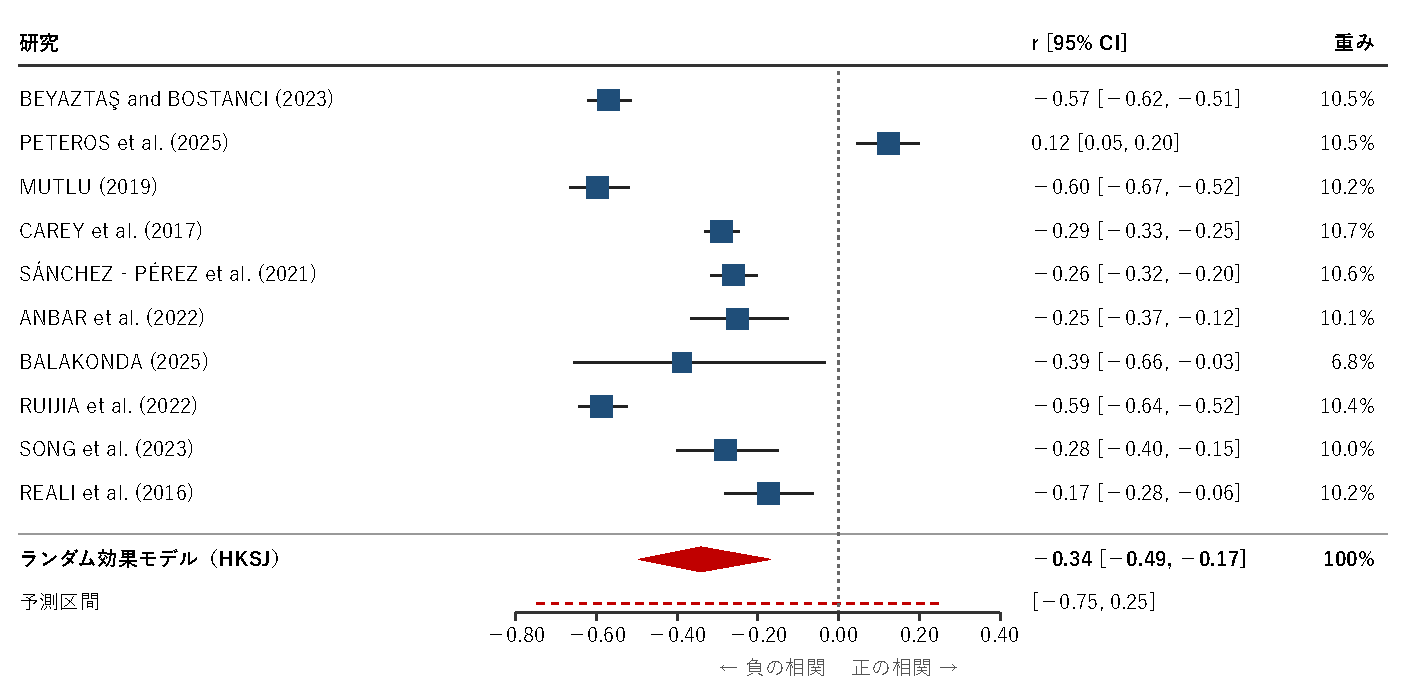
\includegraphics[width=\textwidth]{forest-ja.pdf}\par\vspace{2pt}
{\tablefont\gtfamily 図１\hspace{1em}フォレストプロット\par}{\tablefont 注：四角は各研究の効果量 (大きさは重み)，横線は95\%信頼区間，ひし形は統合値，点線は予測区間を表す．\par}
\end{figure*}
ランダム効果モデルによる統合値は \textit{r} = \ensuremath{-}.34，95\% 信頼区間 [\ensuremath{-}.49, \ensuremath{-}.17]，\textit{t}(9) = \ensuremath{-}4.32，\textit{p} = .002 であった．慣例的な目安では中程度効果にあたる．固定効果モデルによる推定値は \textit{r} = \ensuremath{-}.32 であった．これらの推定値を表３にまとめる．

\secn{3}{4}{異質性}
研究間の異質性は非常に大きかった (\textit{Q}(9) = 288.53，p < .001，\textit{I}² = 96.9\%，\textit{τ}² = 0.063)．95\% 予測区間は \ensuremath{-}.75 から .25 であった．

\secn{3}{5}{下位集団分析と感度分析}
小学校 (１〜６年) では \textit{r} = \ensuremath{-}.44，95\% 信頼区間 [\ensuremath{-}.61, \ensuremath{-}.24] (\textit{k} = 6)，中学校 (７〜９年) では \textit{r} = \ensuremath{-}.11，95\% 信頼区間 [\ensuremath{-}1.00, 1.00] (\textit{k} = 2)，学年混合では \textit{r} = \ensuremath{-}.24，95\% 信頼区間 [\ensuremath{-}.77, .48] (\textit{k} = 2) であり，学校段階間の差は統計的に有意ではなかった (\textit{Q}(2) = 4.84，\textit{p} = .089)．１研究ずつ除いた推定値は \ensuremath{-}.39 から \ensuremath{-}.31 の範囲であった．Egger の検定ではファンネルプロットの非対称性が示されなかった (切片 = \ensuremath{-}1.96，\textit{p} = .680)．下位集団ごとの推定値も表３に示す．

\begin{table*}[tb]
\centering
{\tablefont \gtfamily 表３\hspace{1em}メタ分析の結果\par}\vspace{2pt}
{\tablefont\renewcommand{\arraystretch}{1.12}
\begin{tabular}{lrrrrrrr}
\toprule
モデル & \textit{k} & \textit{N} & \textit{r} & 95\% CI & \textit{p} & \textit{I}² (\%) & \textit{τ}² \\
\midrule
ランダム効果（HKSJ） & 10 & 5389 & \ensuremath{-}.34 & [\ensuremath{-}.49, \ensuremath{-}.17] & .002 & 96.9 & 0.063 \\
固定効果 & 10 & 5389 & \ensuremath{-}.32 & [\ensuremath{-}.34, \ensuremath{-}.29] & < .001 & — & — \\
\hspace{1em}小学校（1〜6年） & 6 & 2731 & \ensuremath{-}.44 & [\ensuremath{-}.61, \ensuremath{-}.24] & .003 & 95.4 & 0.049 \\
\hspace{1em}中学校（7〜9年） & 2 & 642 & \ensuremath{-}.11 & [\ensuremath{-}1.00, 1.00] & .750 & 86.5 & 0.124 \\
\hspace{1em}学年混合 & 2 & 2016 & \ensuremath{-}.24 & [\ensuremath{-}.77, .48] & .151 & 73.5 & 0.006 \\
\bottomrule
\end{tabular}\par}
\vspace{2pt}{\tablefont\noindent 注：\textit{k}＝研究数．HKSJ＝Hartung–Knapp–Sidik–Jonkman 法による信頼区間．95\% 予測区間 [\ensuremath{-}.75, .25]．\par}
\end{table*}
\chap{4}{考察}
ランダム効果モデルによる統合相関は \textit{r} = \ensuremath{-}.34，95\%信頼区間 [\ensuremath{-}.49, \ensuremath{-}.17] であり，慣例的な目安では中程度の負の関連である (表３)．採用した研究では，算数・数学への不安が高い児童生徒ほど，学力が低い傾向があった．10件のうち９件が負の相関を示し，例外は中学２年生を対象に弱い正の相関を示した研究(PETEROS \textit{et al.} 2025)であった．負の相関が最も大きかったのは，トルコと中国の単一学年を対象とした研究(BEYAZTAŞ and BOSTANCI 2023，MUTLU 2019，RUIJIA \textit{et al.} 2022)であり，最大の標本を持つ研究では相関がより小さかった(CAREY \textit{et al.} 2017) (Fig. 1)．

結果は研究間で大きくばらついた (Fig. 1)．異質性は非常に大きく (\textit{I}² = 96.9\%)，95\%予測区間 [\ensuremath{-}.75, .25] は０や弱い正の値を含むほど広かった．このため，統合値をどの教室でも期待できる相関として読むべきではない．不安尺度，学力の測度 (テスト，通知表の成績，教師が報告した成績)，対象となった児童生徒の違いがいずれも寄与している可能性がある (表２) が，今回のデータからは，そのうちどれが違いを説明するのかを述べることはできない．

学校段階別の分析では，小学校の標本 (\textit{r} = \ensuremath{-}.44，\textit{k} = 6) のほうが，中学校の標本 (\textit{r} = \ensuremath{-}.11，\textit{k} = 2) や学年が混在した標本 (\textit{r} = \ensuremath{-}.24，\textit{k} = 2) よりも関連が強い可能性が示された．しかし，学校段階間の差は統計的に有意でなく (\textit{Q}(2) = 4.84，\textit{p} = .089)，中学校の推定値の区間は非常に広く，各下位集団の研究数も少なかった．これらの結果は探索的なものであり，学校段階によって関連が異なる理由については結論を述べない．受動的な比較条件と能動的な比較条件の比較は，この相関の問いには当てはまらなかった．１件ずつ研究を除いた感度分析では統合推定値は \ensuremath{-}.39 から \ensuremath{-}.31 の範囲にあり，全体の結果を単独で決めた研究はなかった．Egger の検定では，ファンネルプロットの非対称性は示されなかった (切片 = \ensuremath{-}1.96，\textit{p} = .680) が，10件の研究では検定の検出力は小さい．

１〜９年生を担当する教師にとって，これらの知見は，成績だけでなく算数・数学に対する児童生徒の気持ちにも目を配ることを示唆する．授業やテストで不安そうに見える児童生徒には，落ち着いた教室，分かりやすい説明，圧力のない練習の機会が役立つかもしれない．同時に，データは相関的なものであるため，不安を下げれば学力が上がることや，学力の低さがそれ自体で不安を生まないことを，今回の結果が示しているわけではない．したがって学校は，不安を注意すべき要因の一つとして捉え，一つの不安得点だけで児童生徒を判断してはならない．

\chap{5}{まとめ}
小・中学校の児童生徒を対象とした10件の研究を通じて，算数・数学への不安が高いほど学力が低い傾向がみられ，統合した相関は \textit{r} = \ensuremath{-}.34 と中程度であった．関連の大きさは研究間で大きく異なり，小学校の標本でより強い可能性があるが，この差は統計的に有意ではなかった．証拠は相関的で，件数が少なく，自動で抽出されたものであるため，教師はこれを児童生徒の不安に目を向ける理由として使うことはできるが，不安を減らすだけで学力が上がることを示すものではない．

本統合にはいくつかの限界がある．採用した研究は10件にとどまり，標本が小さいもの(BALAKONDA 2025)もあれば大きいもの(CAREY \textit{et al.} 2017)もあった．研究は異なる国で行われ，不安尺度も学力の測度も異なっていたため，統合推定値は大まかな要約にとどまる．複数の学年を混ぜた標本があり(CAREY \textit{et al.} 2017，REALI \textit{et al.} 2016)，そのうち１件には対象範囲よりやや年長の生徒が含まれていた(REALI \textit{et al.} 2016)．下位集団には２件しか研究が含まれないものもあり，その推定値は精度が低い．採用した研究はすべて相関的な研究であったため，関係の向きは確かめられない．

研究はオープンアクセスの情報源に限った検索で見つけたものであり，データは本文から自動で抽出した．抽出した数値はすべて本文と照合したが，人による確認は経ていない．また，本文や相関が入手できない，あるいは確実に読み取れないために採用できなかった候補研究も複数あった．研究が複数の結果変数について相関を報告している場合は，主たる学力の測度に対するものを用いており，この選択が結果に影響した可能性がある．以上の理由から，この知見は暫定的なものとして扱うべきである．

加えて，本分析は選別とデータ抽出を言語モデルで自動化しており，抽出した数値は本文との文字列の照合でしか確認していない．数値が本文に存在しても，別の群や別の測定の値を取り違えている可能性は残る．対象はオープンアクセスで本文を取得できた論文に限られ，有料の論文や未刊行の研究は含まれていない．

\chapspaced{付\hspace{1\zw}記}
本論文は，教育情報分析研究会が生成AIを用いて自動で作成した「生成AI論文」である．文献の選別，データの抽出，はじめに・考察・まとめの文章の作成には大規模言語モデル (claude-sonnet-5-5 (Claude Code, local)) を用い，統計量はすべてプログラムで計算した．査読は受けていない．

同じ内容の英語版がある (\url{https://raw.githubusercontent.com/k518-2026/MetaAnalysisToWP/main/reports/2026-10-06-math-anxiety-achievement/paper-en.pdf})．抽出したデータとプログラムは \url{https://github.com/k518-2026/MetaAnalysisToWP} で公開している．

\chapspaced{参考文献}
{\noindent * はメタ分析に含めた研究を示す．\par}
{\small
\par\noindent\hangindent=2\zw\hangafter=1 *ANBAR, N., CHEIE, L. and VISU-PETRA, L. (2022) Math Anxiety, Math Achievement and Gender Differences among Primary School Children and their Parents from Palestine. \textit{International Journal of Learning Teaching and Educational Research}, \textbf{21} (8)：326-334. \url{https://doi.org/10.26803/ijlter.21.8.19}\par
\par\noindent\hangindent=2\zw\hangafter=1 *BALAKONDA, V. (2025) Exploring the Relationship between Mathematics Anxiety, Interest, and Academic Achievement among Secondary School Students. \textit{Journal of Informatics Education and Research}. \url{https://jier.org/index.php/journal/article/view/2800}\par
\par\noindent\hangindent=2\zw\hangafter=1 *BEYAZTAŞ, D. İ. and BOSTANCI, Y. (2023) Investigating the Relationship Between Mathematics Anxiety and Mathematics Achievement of Primary School 4th Grade Students. \textit{Kastamonu Eğitim Dergisi}, \textbf{31} (3)：498-512. \url{https://doi.org/10.24106/kefdergi.1336373}\par
\par\noindent\hangindent=2\zw\hangafter=1 BORENSTEIN, M., HEDGES, L. V., HIGGINS, J. P. T. and ROTHSTEIN, H. R. (2009) \textit{Introduction to Meta-Analysis}. Wiley. \url{https://doi.org/10.1002/9780470743386}\par
\par\noindent\hangindent=2\zw\hangafter=1 *CAREY, E., DEVINE, A., HILL, F. and SZŰCS, D. (2017) Differentiating anxiety forms and their role in academic performance from primary to secondary school. \textit{PLoS ONE}, \textbf{12} (3)：e0174418. \url{https://doi.org/10.1371/journal.pone.0174418}\par
\par\noindent\hangindent=2\zw\hangafter=1 COHEN, J. (1988) \textit{Statistical Power Analysis for the Behavioral Sciences} (2nd ed.). Lawrence Erlbaum Associates\par
\par\noindent\hangindent=2\zw\hangafter=1 DERSIMONIAN, R. and LAIRD, N. (1986) Meta-analysis in clinical trials. \textit{Controlled Clinical Trials}, \textbf{7} (3)：177-188. \url{https://doi.org/10.1016/0197-2456(86)90046-2}\par
\par\noindent\hangindent=2\zw\hangafter=1 EGGER, M., DAVEY SMITH, G., SCHNEIDER, M. and MINDER, C. (1997) Bias in meta-analysis detected by a simple, graphical test. \textit{BMJ}, \textbf{315} (7109)：629-634. \url{https://doi.org/10.1136/bmj.315.7109.629}\par
\par\noindent\hangindent=2\zw\hangafter=1 HARTUNG, J. and KNAPP, G. (2001) A refined method for the meta-analysis of controlled clinical trials with binary outcome. \textit{Statistics in Medicine}, \textbf{20} (24)：3875-3889. \url{https://doi.org/10.1002/sim.1009}\par
\par\noindent\hangindent=2\zw\hangafter=1 HIGGINS, J. P. T. and THOMPSON, S. G. (2002) Quantifying heterogeneity in a meta-analysis. \textit{Statistics in Medicine}, \textbf{21} (11)：1539-1558. \url{https://doi.org/10.1002/sim.1186}\par
\par\noindent\hangindent=2\zw\hangafter=1 INTHOUT, J., IOANNIDIS, J. P. A. and BORM, G. F. (2014) The Hartung-Knapp-Sidik-Jonkman method for random effects meta-analysis is straightforward and considerably outperforms the standard DerSimonian-Laird method. \textit{BMC Medical Research Methodology}, \textbf{14}：25. \url{https://doi.org/10.1186/1471-2288-14-25}\par
\par\noindent\hangindent=2\zw\hangafter=1 *MUTLU, Y. (2019) Math Anxiety in Students With and Without Math Learning Difficulties. \textit{lnternational Electronic Journal of Elementary Education}, \textbf{11} (5)：471-475. \url{https://doi.org/10.26822/iejee.2019553343}\par
\par\noindent\hangindent=2\zw\hangafter=1 *PETEROS, E. D. L., TANDOC, L. B., PALAPAR, M. H., ADLAW, R. C. and FUENTES, C. M. (2025) Mathematics anxiety as a moderator between self-esteem and mathematics achievement among Filipino Grade 8 students. \textit{STEM Education}, \textbf{5} (5)：933-953. \url{https://doi.org/10.3934/steme.2025041}\par
\par\noindent\hangindent=2\zw\hangafter=1 *REALI, F., JIMÉNEZ-LEAL, W., MALDONADO-CARREÑO, C., DEVINE, A. and SZŰCS, D. (2016) Examining the link between math anxiety and math performance in Colombian students. \textit{Revista Colombiana de Psicología}, \textbf{25} (2). \url{https://doi.org/10.15446/rcp.v25n2.54532}\par
\par\noindent\hangindent=2\zw\hangafter=1 *RUIJIA, Z., TALIB, O., BURHANUDDIN, N. A. N. and LI, W. (2022) The Effect of Math Self-Concept and Self-Efficacy on the Math Achievement of Sixth-Grade Primary School Students: The Mediating Role of Math Anxiety. \textit{International Journal of Academic Research in Progressive Education and Development}, \textbf{11} (3). \url{https://doi.org/10.6007/ijarped/v11-i3/14721}\par
\par\noindent\hangindent=2\zw\hangafter=1 *SÁNCHEZ-PÉREZ, N., FUENTES, L. J. and GONZÁLEZ-SALINAS, C. (2021) Assessing math anxiety in elementary schoolchildren through a Spanish version of the Scale for Early Mathematics Anxiety (SEMA). \textit{PLoS ONE}, \textbf{16} (8)：e0255777. \url{https://doi.org/10.1371/journal.pone.0255777}\par
\par\noindent\hangindent=2\zw\hangafter=1 *SONG, S., LI, T., QUINTERO, M. and WANG, Z. (2023) The link between math anxiety and math achievement: The role of afterschool learning. \textit{Journal of Numerical Cognition}, \textbf{9} (3)：418-432. \url{https://doi.org/10.5964/jnc.11325}\par
}
\chapspaced{Summary}
{\setlength{\parindent}{1\zw}\noindent Mathematics anxiety is a feeling of tension about mathematics, and understanding how it relates to achievement helps teachers in primary and lower secondary schools support their students. Using an automated workflow in which every extracted number was verified against the full text, 10 open-access studies (\textit{N} = 5389) were pooled with a random-effects model. The pooled effect was \textit{r} = \ensuremath{-}.34, 95\% CI [\ensuremath{-}.49, \ensuremath{-}.17], with \textit{I}² = 96.9\%. Higher mathematics anxiety was generally linked with lower achievement, but the size of the link varied widely, so teachers should treat it as a correlation rather than a proven cause.\par
KEYWORDS: META-ANALYSIS, MATHEMATICS ANXIETY, MATHEMATICS ACHIEVEMENT, PRIMARY EDUCATION, LOWER SECONDARY EDUCATION, CORRELATION\par}
\end{document}
